\documentclass[12pt,letterpaper]{article}


\usepackage[top=1in, 
		    bottom=1in,
		    left=1in,
		    right=1in]{geometry}
\usepackage{setspace}	% makes the \singlespacing, \onehalfspacing, and \doublespacing commands available
% \usepackage[en-US]{datetime2}
% \DTMlangsetup{showdayofmonth=false}
% \usepackage{titlesec}
\usepackage{listings}	% allows for placing programming code to be displayed correctly
\usepackage{siunitx}	% units
\usepackage{amsmath}
\usepackage{amsfonts}
\usepackage{amssymb}
\usepackage{graphicx}
\usepackage{booktabs}
\usepackage{multirow}
\usepackage{pgfplots}
\pgfplotsset{compat=newest}
\usepackage{tikz}
%\usetikzlibrary{shapes.geometric}
% \usepgfplotslibrary{external} 
% \tikzexternalize[prefix=pdfimages/,
% 		        mode=list and make]
\usepackage{caption}
\usepackage[list=true,
		     listformat=simple]{subcaption}
%\usepackage{cleveref}	% this should really go last
\usepackage[
	colorlinks,
	linkcolor=black,
	citecolor=black,
	plainpages=false,
	pdfpagelabels]{hyperref}
% \usepackage[all]{hypcap}
\usepackage{cleveref}
\input{./formatting}
\newcommand{\mymder}[2]{\ensuremath{\frac{\mathrm{D}#1}{\mathrm{D}#2}}}
\newcommand{\mypder}[2]{\ensuremath{\frac{\partial #1}{\partial #2}}}
\newcommand{\mypdertwo}[2]{\ensuremath{\frac{\partial^2 #1}{\partial #2^2}}}
\newcommand{\mymdervec}[1]{\ensuremath{mypder{#1}{t} + }}
\newcommand{\myder}[2]{\ensuremath{\frac{d#1}{d#2}}}
\newcommand{\mydiv}[1]{\ensuremath{\nabla \cdot {#1}}}
\newcommand{\myfrac}[2]{\ensuremath{^{#1}\!/_{#2}}}
\newcommand{\myfunc}[2]{\ensuremath{#1 \left( #2 \right)}}
\newcommand{\myparen}[1]{\ensuremath{\left( #1 \right)}}
\newcommand{\mybrack}[1]{\ensuremath{\left[ #1 \right]}}
\newcommand{\mybrace}[1]{\ensuremath{\left\{ #1 \right\}}}
\newcommand{\mysin}[1]{\ensuremath{\myfunc{\mathrm{sin}}{#1}}}
\newcommand{\mycos}[1]{\ensuremath{\myfunc{\mathrm{cos}}{#1}}}
\newcommand{\myexp}[1]{\ensuremath{\myfunc{\mathrm{exp}}{#1}}}
\newcommand{\myint}[4]{\ensuremath{\int_{#1}^{#2} {#3} d {#4}}}


\newcommand{\Rld}{\ensuremath{\mathit{Re}}}
\newcommand{\St}{\ensuremath{\mathit{St}}}
\newcommand{\Prn}{\ensuremath{\mathit{Pr}}}
\newcommand{\Sc}{\ensuremath{\mathit{Sc}}}
\newcommand{\Sh}{\ensuremath{\mathit{Sh}}}
\newcommand{\Nu}{\ensuremath{\mathit{Nu}}}
\newcommand{\Bi}{\ensuremath{\mathit{Bi}}}


\let\textacute\'
\let\textgrave\`


\newcommand{\includetikz}[2]{%
    \tikzsetnextfilename{#2}%
    \input{#1#2.tex}%
}

\begin{document}

\noindent
MECH 131A Homework 2

\noindent
Assigned date: October $8^{\mathrm{th}}$, 2024

\noindent
Due date: October $18^{\mathrm{th}}$, 2024

\subsubsection*{Instructions}
\begin{enumerate}
	\item Indicate the names of your study group members.
	\item Draw a sketch of the problem.
	\item If using a specific solution methodology is specified, please include a copy of the Python/MATLAB script.
	\item If using a specific solution methodology is \textit{not} specified, please include a copy of your computationally methodology.
\end{enumerate}


\subsubsection*{Problem Set}
\begin{enumerate}

\item Redo the example problem from class with the water pipes and radiative heating.
	
	\begin{enumerate}
		\item Instead of assuming the thin layer of aluminum is held at \SI{60}{\celsius} where it touches the water pipe, assume there is a resistance network connecting the flowing water to the thin layer of aluminum.
			Your solution should depend on a \Bi~that depends on a total resistance instead of just a heat transfer coefficient.
			Comment on the effect of the \Bi~on the solution.
			When does it approximate the solution assuming thin layer of aluminum is held at \SI{60}{\celsius} where it touches the water pipe?
			When does it not?
		\item In this part you will get a more accurate solution by including the temperature dependence of the radiative heat transfer.
			\begin{enumerate}
				\item Using the results from the solution in class, estimate the temperature of the heated surface radiating to the aluminum plate.
					What radiating temperature, $T_r$, gives a value of \SI{800}{\watt\per\square\meter} on average over the surface of the fin?
					Use emissivity from both highly polished and highly anodized aluminum.
				\item Derive the appropriate fin equation using the Stefan-Boltzmann law for grey surfaces instead of Newton's law of cooling.
				
				\begin{equation*}
					q'' = \epsilon \sigma \left( T_r^4 - T^4 \right)
				\end{equation*}
				
				\item Integrate the equation numerically and compare to the solution above when you assumed $q'' = \SI{800}{\watt\per\square\meter}$ for a variety of \Bi and both finishes of aluminum.
					Comment on the differences.
			\end{enumerate}
	\end{enumerate}

% Superposition Question
\item For the boundary conditions listed below, plot a contour of the temperature profile and heat flow lines.
	Discuss and explain the general shape of the temperature contours and the heat flow lines.
	Feel free to base your work on the script shown in class and posted at the class GitHub repository.

	\begin{enumerate}
		\item $\myfunc{\theta}{x, y = 0} = 0$, $\myfunc{\theta}{x, y = W} = 1$, $\myfunc{\theta}{x = 0, y} = 0$, $\myfunc{\theta}{x = L, y} = 0$
		\item $\myfunc{\theta}{x, y = 0} = 0$, $\myfunc{\theta}{x, y = W} = 1$, $\myfunc{\theta}{x = 0, y} = 1$, $\myfunc{\theta}{x = L, y} = 0$
		\item $\myfunc{\theta}{x, y = 0} = 1$, $\myfunc{\theta}{x, y = W} = 1$, $\myfunc{\theta}{x = 0, y} = 0$, $\myfunc{\theta}{x = L, y} = 0$
		\item $\myfunc{\theta}{x, y = 0} = 1$, $\myfunc{\theta}{x, y = W} = 1$, $\myfunc{\theta}{x = 0, y} = 1$, $\myfunc{\theta}{x = L, y} = 0$
	\end{enumerate}

%% Propellant Tank Fin analysis
%\item You are part of a team that analyzes cryogenic propellant tank temperatures and pressures for a rocket.
%	Your team maintains a thermal lumped parameter model used to predict tank conditions throughout flight.
%	There is concern about the effect of the heat loss through wall of the tank near the top where the gas is (commonly called ``the ullage'').
%	Your task is to develop a model to more accurately predict the net heat transfer to the vehicle.
%	For the analysis below, you can assume the heat transfer coefficients for a given volume of fluid are the same at all interfaces.
%
%	\begin{enumerate}
%		\item Derive the governing equation for the thin walls shown in the figure below.
%			Assume you can ignore the transverse temperature change across the tank walls.
%		\item There are two possible far-field boundary conditions for the tank walls.
%			Describe the boundary conditions for both:
%		
%		\begin{enumerate}
%			\item the cryogenic liquid is boiling,
%			\item the cryogenic liquid is not boiling.
%		\end{enumerate}
%
%		\item Solve the inter-linked system of ordinary differential equations for both sets of assumed boundary conditions from above, and the range of heat transfer coefficient values shown in the figure below.
%		Make sure there is continuity of temperature and conservation of energy at the various fin junctions.
%
%		\item Comment on how changing the height of the ullage affects the heat transfer to the ullage.
%			Is there an optimum height to minimize the heat transfer to the ullage?
%			How does this compare to the default heat transfer values used by the team?
%
%		\item If the default model currently used by the team does not account for the fin-like effects of the tank wall and only accounts for heat transfer in across the tank walls, comment on the effect of using the fin-models.
%			How do they affect the net heat transfer to the vehicle?
%			Under what conditions is the effect the most pronounced?
%			Answer these in the context of the analysis done for the previous two bullet points (accounting for the range in heat transfer coefficients and height of the ullage), also looking at the other heat transfers described in the figure below.
%	\end{enumerate}
%
%
%\begin{figure}[!htpb]
%	\centering
%	% https://cremeronline.com/LaTeX/minimaltikz.pdf is a great primer for tikz

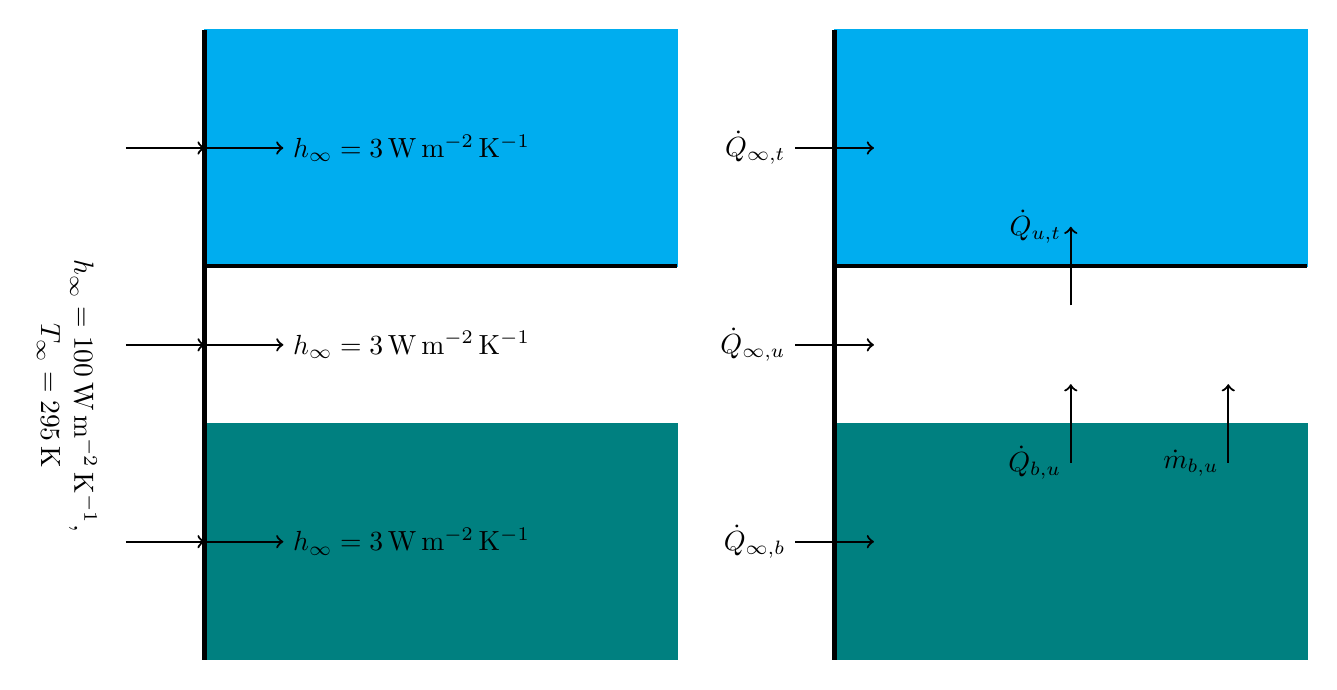
\begin{tikzpicture}
    %%  Draw Tank with htc Labels
    % Draw Tank
    \draw [fill=teal, draw=teal] (0,0) rectangle (6, -3);
    \draw [fill=cyan, draw=cyan] (0,2) rectangle (6,5);
    
    \draw [ultra thick] (0, -3) -- (0, 5);
    \draw [ultra thick] (0, 2) -- (6, 2);

    % Heat Transfer Coefficients
    \draw [->, thick] (-1, -1.5) -- (0, -1.5);
    \draw [->, thick] (-1, 1) -- (0, 1);
    \draw [->, thick] (-1, 3.5) -- (0, 3.5);
    \node [align=center, left, rotate=-90] at (-1.75, -1.5) {$h_{\infty} = \SI{100}{\watt\per\square\meter\per\kelvin}$, \\ $T_{\infty} = \SI{295}{\kelvin}$};
%    % Ambient to tank wall (bottom propellant)
%	\draw [->, thick] (-1, -1.5) -- (0, -1.5);
%    \node [align=center, left] at (-1, -1.5) {$h_{\infty} = \numrange{10}{100}~\si{\watt\per\square\meter\per\kelvin}$, \\ $T_{\infty} = \SI{295}{\kelvin}$};
%   % Ambient to tank wall (ullage propellant)
%	\draw [->, thick] (-1, 1) -- (0, 1);
%    \node [align=center, left] at (-1, 1) {$h_{\infty} = \numrange{10}{100}~\si{\watt\per\square\meter\per\kelvin}$, \\ $T_{\infty} = \SI{295}{\kelvin}$};
%    % Ambient to tank wall (top propellant)
%    \draw [->, thick] (-1, 3.5) -- (0, 3.5);
%    \node [align=center, left] at (-1, 3.5) {$h_{\infty} = \numrange{10}{100}~\si{\watt\per\square\meter\per\kelvin}$, \\ $T_{\infty} = \SI{295}{\kelvin}$};
    % Tank wall to bottom propellant
    \draw [->, thick] (0, -1.5) -- (1, -1.5);
    \node [align=center, right] at (1, -1.5) {$h_{\infty} = \SI{3}{\watt\per\square\meter\per\kelvin}$};
    % Tank wall to ullage
    \draw [->, thick] (0, 1) -- (1, 1);
    \node [align=center, right] at (1, 1) {$h_{\infty} = \SI{3}{\watt\per\square\meter\per\kelvin}$};
    % Tank wall to top propellant
    \draw [->, thick] (0, 3.5) -- (1, 3.5);
    \node [align=center, right] at (1, 3.5) {$h_{\infty} = \SI{3}{\watt\per\square\meter\per\kelvin}$};
    
   
    %%  Draw Tank with HT labels
    % Draw Tank
    \draw [fill=teal, draw=teal] (8,0) rectangle (14, -3);
    \draw [fill=cyan, draw=cyan] (8,2) rectangle (14,5);
    
    \draw [ultra thick] (8, -3) -- (8, 5);
    \draw [ultra thick] (8, 2) -- (14, 2);
    
    % HT
    % Ambient to bottom propellant
    \draw [->, thick] (7.5, -1.5) -- (8.5, -1.5);
    \node [left] at (7.5, -1.5) {$\dot{Q}_{\infty, b}$};
    % Ambient to ullage
    \draw [->, thick] (7.5, 1) -- (8.5, 1);
    \node [left] at (7.5, 1) {$\dot{Q}_{\infty, u}$};
    % Ambient to top propellant
    \draw [->, thick] (7.5, 3.5) -- (8.5, 3.5);
    \node [left] at (7.5, 3.5) {$\dot{Q}_{\infty, t}$};
    % Bottom propellant to ullage
    \draw [->, thick] (11, -0.5) -- (11, 0.5);
    \node [left] at (11, -0.5) {$\dot{Q}_{b, u}$};
    \draw [->, thick] (13, -0.5) -- (13, 0.5);
    \node [left] at (13, -0.5) {$\dot{m}_{b, u}$};
    % Ullage to top propellant
    \draw [->, thick] (11, 1.5) -- (11, 2.5);
    \node [left] at (11, 2.5) {$\dot{Q}_{u, t}$};
    
\end{tikzpicture}
%	\caption{The figure on the left shows the expected ranges for the heat transfer coefficient when the there is \textit{no} boiling on the inside walls of the tank.
%		The figure on the right shows all the heat transfers currently accounted for in the thermal model.
%		If you need dimensional values for the tank, use the Saturn V second stage (S-II) which is \SI{10}{\meter} in diameter and had a hydrogen-LOX propellant mixture.
%		You can assume the hydrogen and LOX are saturated at ambient conditions for this analysis.}
%\end{figure}


% 2D Fin
\item In this question you will analytically describe the applicability of the thin fin approximation. 

	\begin{enumerate}
		\item Show that the 2D steady equation,
			
			\begin{equation*}
				\mypdertwo{\theta}{x} + \mypdertwo{\theta}{y} = 0,
			\end{equation*}
			
			is equivalent to
			
			\begin{gather*}
				\mypdertwo{Y}{y} + \lambda^2 Y = 0, \\
				\mypdertwo{X}{x} - \lambda^2 X = 0, \\
			\end{gather*}
			
			when assuming separation of variables, i.e. $\myfunc{\theta}{x, y} = \myfunc{X}{x} \myfunc{Y}{y}$.
			
		\item There is a semi-infinite rectangular region $2t$ wide with the following boundary conditions:

			\begin{gather*}
				\myfunc{\theta}{x = 0, y} = \theta_b, \quad \myfunc{\theta}{x \to \infty, y} = 0, \\
				\left. \mypder{\theta}{y} \right|_{x, y = 0} = 0, \quad -k \left. \mypder{\theta}{y} \right|_{x, t} = h \myfunc{\theta}{x, t}.
			\end{gather*}
		
			Briefly describe the use of symmetry in the boundary conditions.
		
		\item Use the three homogenous boundary conditions to show that the eigenfunctions for the boundary conditions above are described by
			
			\begin{equation*}
				\theta_n = C_n \myexp{- \lambda_n x} \mycos{\lambda_n y},
			\end{equation*}
			
			where
			
			\begin{equation*}
				\mathrm{tan} \left( \lambda_n t \right) = \Bi / \lambda_n t, \quad \Bi= h t / k .
			\end{equation*}
		
		\item Show that using the remaining non-homogeneous boundary condition,
		
			\begin{equation*}
				\theta_b = \sum_{n = 1}^\infty C_n \mycos{\lambda_n y}
			\end{equation*}
			
			results in
			
			\begin{equation*}
				C_n = \frac{2 \theta_b \mysin{\lambda_n t}}{\lambda_n t + \mysin{\lambda_n t} \mycos{\lambda_n t}}.
			\end{equation*}
			
			You now have the analytical solution for an infinite fin that includes the temperature change across the fin.
			
			\begin{equation*}
				\frac{\theta}{\theta_b} = 2 \sum_{n=1}^{\infty} \frac{\mysin{\lambda_n t}}{\lambda_n t + \mysin{\lambda_n t} \mycos{\lambda_n t}} \myexp{- \lambda_n x} \mycos{\lambda_n y}
			\end{equation*}
		
		\item Comment on the required number of terms for accuracy to ensure accuracy of the equation above for $\Bi = 1 \times 10^{-3}$ and $\Bi = 1 \times 10^3$.
		Why does one require more terms?
		Feel free to use the script at the class GitHub repository to generate the sequence of roots of the transcendental equation describing the values of $\lambda_n$.
		
		\item Using the base heat transfer as the measure of comparison, comment on the accuracy of the thin-fin approximation as a function of \Bi.
		Plot an appropriate normalized error between the heat flux from the base of the fin for the infinite thin-fin and 2D solutions for $\Bi = 0.001, 0.01, 0.1, 1, 10, 100, 1000$ with logarithmically scaled axes.
		When does the error become acceptably small?
		
		\item Finally, comment on the meaning and implications of the \Bi~for fins.

	\end{enumerate}


\end{enumerate}


\end{document}